\documentclass[11pt]{article}

\usepackage[hyperfootnotes=false]{hyperref}
\usepackage[margin=1in]{geometry}                                              
\usepackage{amsmath,amsthm,amssymb}      
\usepackage{titlesec}                                                         
\usepackage{bm}        
\usepackage{cprotect}                                
\usepackage{savetrees} 
\usepackage{bbold}
\usepackage{abstract}
                                          
\usepackage{graphicx}                                      
\graphicspath{{../figures/}, {../figures/growthrates/}}

\usepackage{biblatex}
\bibliography{bib.bib}

\titleformat{\subsection}[runin]
{\normalfont\large\bfseries}{\thesubsection}{1em}{}

\renewcommand{\bf}{\mathbf}
\renewcommand{\cal}{\mathcal}
\newcommand{\pd}[2]{\frac{\partial #1}{\partial #2}}
\newcommand{\pdn}[3]{\frac{\partial^{#3} #1}{\partial #2^{#3}}}
\newcommand{\pdop}[1]{\frac{\partial}{\partial #1}}
\newcommand{\nd}[2]{\frac{d #1}{d #2}}
\newcommand{\ndn}[3]{\frac{d^{#3} #1}{d #2^{#3}}}
\newcommand{\ndop}[1]{\frac{d}{d #1}}
\newcommand{\dt}{\frac{d}{dt}}
\newcommand{\grad}{\bm\nabla}
\newcommand{\cross}{\times}
\newcommand{\curl}{\grad\cross}
\newcommand{\imp}{\Longrightarrow\quad}
\newcommand{\abs}[1]{\left|#1\right|}
\newcommand{\half}{\frac{1}{2}}
\newcommand{\third}{\frac{1}{3}}
\renewcommand{\th}[1]{\frac{1}{#1}}
\renewcommand{\k}{4\pi\epsilon_0}
\newcommand{\eps}{\epsilon_0}
\newcommand{\intt}{\int_{t_1}^{t_2}}
\newcommand{\inti}{\int_{-\infty}^{+\infty}}
\newcommand{\ex}[1]{\left\langle #1 \right\rangle}
\newcommand{\oom}[1]{\times 10^{#1}}
\renewcommand{\d}{\delta}
\newcommand{\e}{\text{e}}
\renewcommand{\l}{\ell}
\newcommand{\om}{\omega}
\newcommand{\h}{\hbar}
\newcommand{\ket}[1]{\left|#1\right\rangle}
\newcommand{\bra}[1]{\left\langle#1\right|}
\newcommand{\braket}[2]{\left\langle#1\middle|#2\right\rangle}
\newcommand{\brakett}[3]{\left\langle#1\middle|#2\middle|#3\right\rangle}
\newcommand{\nn}{\nonumber\\}

\begin{document}

\title{Entanglement Dynamics in Random Unitary Circuits}
\author{Charles Stahl}

\maketitle

\begin{abstract}
	Quantum circuits provide simple toy systems to analyze entanglement growth and operator spreading in many-body systems. We study the behavior of these systems under various architectures.
\end{abstract}

\tableofcontents

\newpage

\section{Introduction} \label{sec:intro}

\section{Circuit Architectures} \label{sec:arch}

\section{Ergodicity and Stability} \label{sec:erg}

A Markov process is one in which the future state depends only on the current state, not the past. Label the states $s_i$ and define $p_{i,t}$ as the probability that the system is in state $s_i$ at time $t$. For Markov processes it is possible to define the transition matrix... Since the product of the transition matrix and a probability vector gives the probabilities at the next time step, the transition matrix for $T$ time steps is just $P^T$. Under certain conditions\footnote{Figure these out.} the multi-step transition matrix approaches a constant matrix with all columns equal to the same vector $v^*$,
\begin{align}
\lim\limits_{T\to \infty}P^T = P^* = \begin{bmatrix}
\vdots & \vdots &  & \vdots\\
v^* & v^* & \cdots & v^*\\
\vdots & \vdots &  & \vdots\\
\end{bmatrix}.
\end{align}
Then the probability after a long time is the vector $v^*$ for any initial state.

\subsection{Stable State in Random Architecture} \emph{} \label{subs:randstate}

For the 1-stair circuit, the transition matrix is the matrix product of single-site transition matrices $P_{N} = \prod_NP_{1}\otimes$, where the single-state transition matrix is
\begin{align}
P_1 = \begin{bmatrix}
1-\frac{1+m}{2}\Gamma & \frac{1+m}{2}\Gamma & 0 & 0\\
0 & 1-\Gamma & \Gamma & 0\\
\frac{1-m}{2}\Gamma & 0 & 1-\Gamma & \frac{1+m}{2}\Gamma\\
0 & \frac{1-m}{2}\Gamma & 0 & 1 - \frac{1-m}{2}\Gamma
\end{bmatrix}.
\end{align}
The equilibrium state is
\begin{align}
v^* = \begin{pmatrix}
content...
\end{pmatrix}
\end{align}

\section{Behavior Ignoring Correlations} \label{sec:anal}

Under certain approximations the entanglement entropy behaves analytically. One important approximation (mentioned in section \ref{sub:randgates}) is that the Hilbert space at each site is large enough that any gate will in general maximally entangle the two sites on which it acts. Other simplifying assumptions include ignoring correlations in ups and downs and ignoring second- and higher-order derivatives in $S(x,t)$. Combining these two assumptions, we arrive at uncorrelated entropy environments, which may be described only by their slope, $m$.

\subsection{Small Stairs} \label{sub:smallstairs} \emph{}

The smallest stairs are 1-stairs, which are just individual gates. For an entropy surface with constant slope $m$ and no correlations, each step from one site to the next has probability $\frac{1+m}{2}$ of being up and $\frac{1-m}{2}$ of being down. Consider a gate operating on site $n$ at time $t$. For the gate to increase the entropy $S(n)$, it must be the case that $S(n)<S(n-1), S(n+1)$. The probability of this is $\frac{1+m}{2} \frac{1-m}{2} = \frac{1-m^2}{4}$. In this case we have $S(n,t+1)=S(n,t)+2$, because the gate increases the entropy to be great than that of its neighbors. Then if the gates arrive with a rate $\Gamma$, we have
\begin{align}
\pd{S}{t} = \Gamma\frac{1-m^2}{2}.
\end{align}
Useful checks of this formula are that the entropy does not increase at maximal or minimal slope $m=1,-1$, and that at $m=0$, $\pd{S}{t}=\Gamma/2$, half the brickwork value. The latter rate makes sense because in the case of the brickwork circuit all gates are guaranteed to raise the entropy, while here only half will have an effect.

2-stairs consist of one gate acting at site $n$ and one at site $n+1$. The entropy production of these gates is affected by the slope between them and the two slopes on either side. There are 8 possible configurations of those three slopes, but only 4 result in entropy growth, as shown in table~\ref{tab:2stair}. Together, they result in an average growth
\begin{align}
\pd{S}{t} = \Gamma\frac{1-m^2}{2}\frac{5+m}{4},
\end{align}
where $\Gamma$ is the rate of gates, so the rate of 2-stairs is $2\Gamma$.

\begin{table}
	\centering
	\begin{tabular}{ccc}
		Configuration & Probability                    & Productivity\\
		$d\,u\,d$     & $\frac{1-m^2}{4}\frac{1-m}{2}$ & 2\\
		$d\,u\,u$     & $\frac{1-m^2}{4}\frac{1+m}{2}$ & 4\\
		$d\,d\,u$     & $\frac{1-m^2}{4}\frac{1-m}{2}$ & 2\\
		$u\,d\,u$     & $\frac{1-m^2}{4}\frac{1+m}{2}$ & 2
	\end{tabular}
	\caption{The four configurations that result in entropy growth for 2-stairs, their relative proportions assuming an uncorrelated entropy distribution, and the growth in entropy generated by a 2-stair falling on that configuration.}
	\label{tab:2stair}
\end{table}

\subsection{Larger Stairs} \emph{} \label{sub:largestairs}

We can determine the growth rate for arbitrary length stairs through a recursive relationship. Consider a staircase made of $n$ gates. Its growth rate will be proportional to the gate rate normalized by the number of gates per stair, so we can write
\begin{align}
\pd{S}{t} = \frac{\Gamma}{n}R_n(m), \label{eqn:growthrate}
\end{align}
where $R_n(m)$ is the average entropy production of an $n$-stair. To find an equation for $R_n(m)$, note that the first $n-1$ gates have the same entropy production as the $(n-1)$-stair. Then the $n$th gate will produce another 2 units of entropy if the last step is up, but not if all $n+1$ steps are up. This is captured by the recursive formula
\begin{align}
R_n(m) = R_{n-1}(m)+2\frac{1+m}{2} - 2\left(\frac{1+m}{2}\right)^{n+1}. \label{eqn:raterecur}
\end{align}
Figure~\ref{fig:growthrates} contains a graph of some growth rates $\th{n}R_n(m)$ as a function of $m$.

\begin{figure}
	\centering
	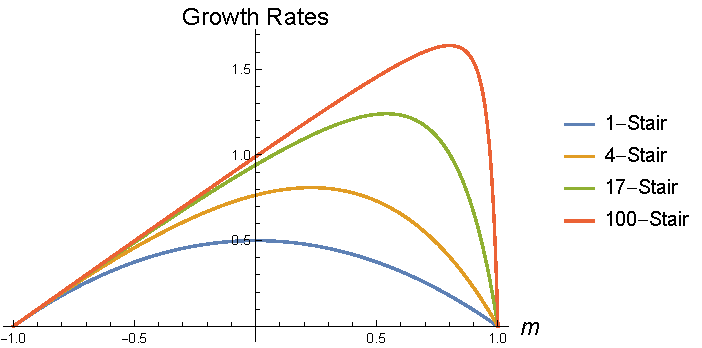
\includegraphics[width=.5\textwidth]{analrates.png}
	\caption{Growth rates for 1-, 4-, 17-, and 100-stairs as a function of slope $m$. As stair length increases, the growth rate asymptotes to the function $\pd{S}{t} = m+1$.}
	\label{fig:growthrates}
\end{figure}

Note that with increasing stair length the growth rate asymptotes to the function $\pd{S}{t} = m+1$. There are two ways to reach this behavior. The first, which matches the order of the current reasoning, is to start with infinite spatial support and take the stair length $n\to\infty$. Alternatively, start with a finite spin chain with length $N$ and periodic boundary conditions, and set the stair length to $N$. Now a single gate acts on site $1,2,3\dots N$, before wrapping around to act at site 1 again. 

The maximal growth rate occurs when the slope is near-maximal, with only a single down step. This corresponds to a slope of $\frac{N-2}{N}$. Then with only a single local minimum in the entropy function, the local minimum moves one site to the right with each gate. Every gate that acts raises the entropy, resulting in an entropy gain of 2 per gate. Of course for a slope of 1, there is still no entropy generation.

If there are 2 down steps, for a slope of $\frac{N-4}{N}$, the entropy generation is almost the same. One local minimum still moves to the right with the leading edge of the staircase. However, once per staircase (once every $N$ gates), one down step is next to the other down step. This results in no entropy growth for that step, for an average entropy gain of $2\frac{N-1}{N}$. Further discussion of the dynamics with near-maximal slope appear in section~\ref{sec:nearmax}.

This pattern continues as the slope decreases. With $\l$ down steps, the slope is $\frac{N-2\l}{N}$ and the average growth rate is $2\frac{N-\l}{N} = m+1$. At $m = -1$ there is no growth, as expected. At $m=0$, the growth rate is 1, the same as in the brickwork model. With no slope, the steps alternate between up and down, so that half of the gates in any stair are effective, explaining the connection to the brickwork model.

\section{Numerical Simulation} \label{sec:num}

To simulate the entropy growth in infinite spin chains with non-zero slope, we used finite chains with periodic boundary conditions, where one end of the chain is attached to the other with an offset. For 1-stairs (the random architecture), the measured growth rate is slightly larger than predicted, seen in figure~\ref{fig:1stair}.
\begin{figure}
	\centering
	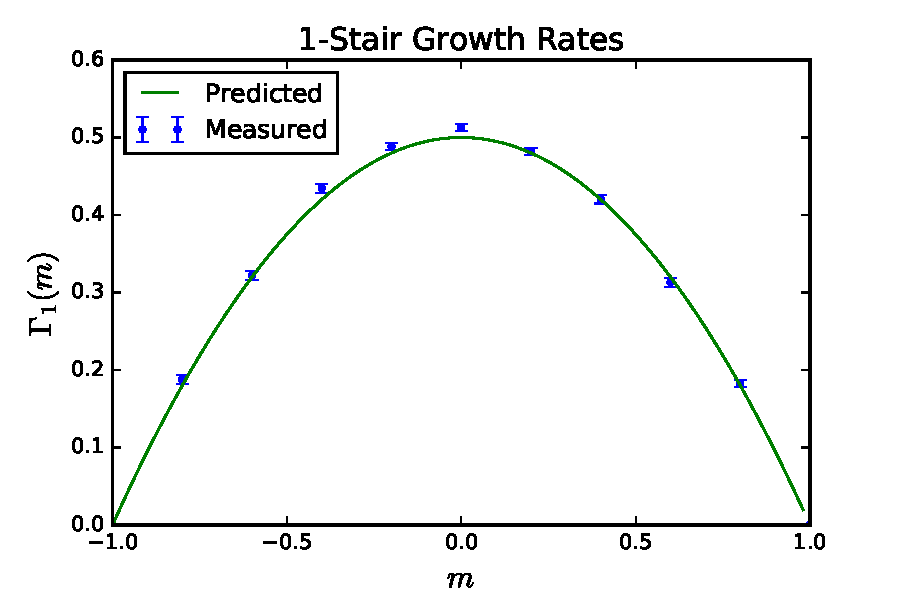
\includegraphics[width=.5\textwidth]{1stairRates.pdf}
	\caption{\textbf{Measured and analytic growth rates} for the 1-stair architecture. Note that the measured rate is slightly higher. Since the assumption of un-correlation is exact for 1-stairs, this difference is assumed to be due to second order derivatives in the slope and finite length effects.}
\end{figure}
There are two main differences between the analytic and measured setups. For the analytic result, the chain is infinite and the entropy function is assumed to be linear and uncorrelated. 





\printbibliography

\end{document}
